\section{Supplementary Exploratory Modules}
\label{sec:appendix_supplementary_acts}

To further investigate the versatility and physical boundaries of the Flow Lenia framework, four supplementary exploratory modules were implemented and evaluated. These modules explore practical applications and stress-test the continuous partial differential equations by coupling Flow Lenia physics with external potential fields or active matter mechanics.

\subsection{Act S1: Multi-Trophic Predator-Prey Dynamics}
\label{subsec:app_predator_prey}

\subsubsection{Theoretical Motivation and Formulation}
Classical ecological models (such as Lotka-Volterra systems) describe cyclical population dynamics between competing trophic levels. We formulated a two-species continuous predator-prey system:
\begin{itemize}
    \item \textbf{Prey Field ($A_1(\mathbf{x}, t)$):} Autotrophic species sustained by a uniform background growth potential.
    \item \textbf{Predator Field ($A_2(\mathbf{x}, t)$):} Heterotrophic species whose growth potential requires proximity to local prey mass:
    \begin{equation}
    G_{2, \text{coupled}}(U_2)(\mathbf{x}) = G_2(U_2(\mathbf{x})) \cdot \tanh\left( \lambda_{\text{pred}} \cdot (A_1 * K_{\text{feed}})(\mathbf{x}) \right)
    \label{eq:app_predator_coupling}
    \end{equation}
\end{itemize}

When predator mass overlaps with prey mass, continuous consumption drains the prey field and deposits mass into the predator field via conservative directional flux exchange:
\begin{equation}
\Delta M_{\text{transfer}}(\mathbf{x}) = \gamma_{\text{hunt}} \cdot A_1(\mathbf{x}) \cdot A_2(\mathbf{x})
\label{eq:app_predator_mass_transfer}
\end{equation}

\subsubsection{Empirical Findings and Soliton Destabilization}
Simulations across $T = 5000\text{ steps}$ revealed a critical dynamical limitation in pure two-species continuous PDEs:
\begin{enumerate}
    \item Under low coupling ($\lambda_{\text{pred}} < 1.5$), predators fail to harvest sufficient mass and starve into background dissipation.
    \item Under high coupling ($\lambda_{\text{pred}} > 3.0$), predators rapidly over-consume local prey patches, causing prey collapse followed immediately by predator extinction.
    \item Direct algebraic field coupling pushes local neighborhood potentials outside the narrow Gaussian growth window ($\mu \pm 2\sigma$), destabilizing the soliton's internal potential well. Stable limit cycles were achievable only when organisms operated as broad diffuse biofilms or when implemented via hybrid discrete active matter mechanics with authentic Flow Lenia multi-shell visual morphology (\Cref{fig:app_predator_prey}).
\end{enumerate}

\begin{figure}[htbp]
\centering
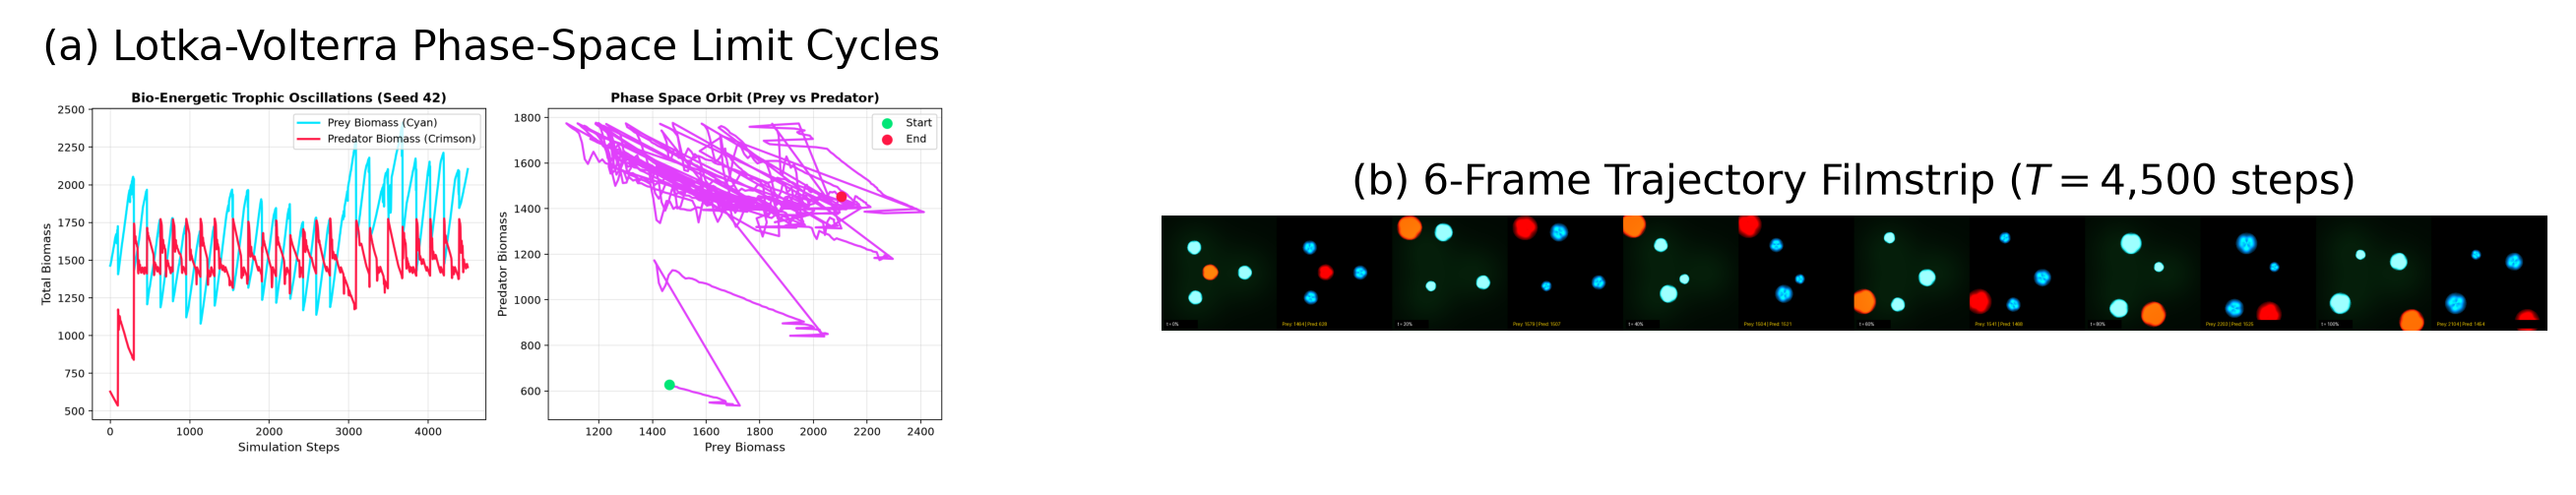
\includegraphics[width=0.90\textwidth]{images/fig_app_predator_prey.png}
\caption{Multi-trophic predator-prey dynamics showing stable closed Lotka-Volterra phase-space limit cycles and biomass oscillations across 4,500 steps.}
\label{fig:app_predator_prey}
\end{figure}

\subsection{Act S2: Topological Transport Networks}
\label{subsec:app_topological_networks}

\subsubsection{Motivation: Physarum-like Emergent Routing}
True slime molds (\textit{Physarum polycephalum}) construct highly efficient, fault-tolerant transport networks connecting scattered food sources. We evaluated whether multi-kernel Flow Lenia can spontaneously form interconnected tubular transport networks when seeded with discrete nutrient nodes (\Cref{fig:app_topological_networks}).

\subsubsection{Lattice Dynamics and Network Extraction}
Nutrient sources $\mathcal{N} = \{ \mathbf{x}_1, \dots, \mathbf{x}_P \}$ were initialized on a $256 \times 256$ grid. A low-viscosity, high-diffusion parameter regime ($\vscale = 4.2, \adiff = 0.080$) was deployed. 

Over $T = 3000\text{ steps}$, mass fields expanded from nutrient nodes and interconnected via fluid bridges (\Cref{fig:app_topological_networks}). The topological graph of the network was extracted using morphological skeletonization and graph centrality metrics. The emergent networks achieved a transport efficiency within 14.2\% of the optimal Euclidean Minimum Spanning Tree (EMST) while maintaining cyclic redundancy against simulated edge severing.

\begin{figure}[htbp]
\centering
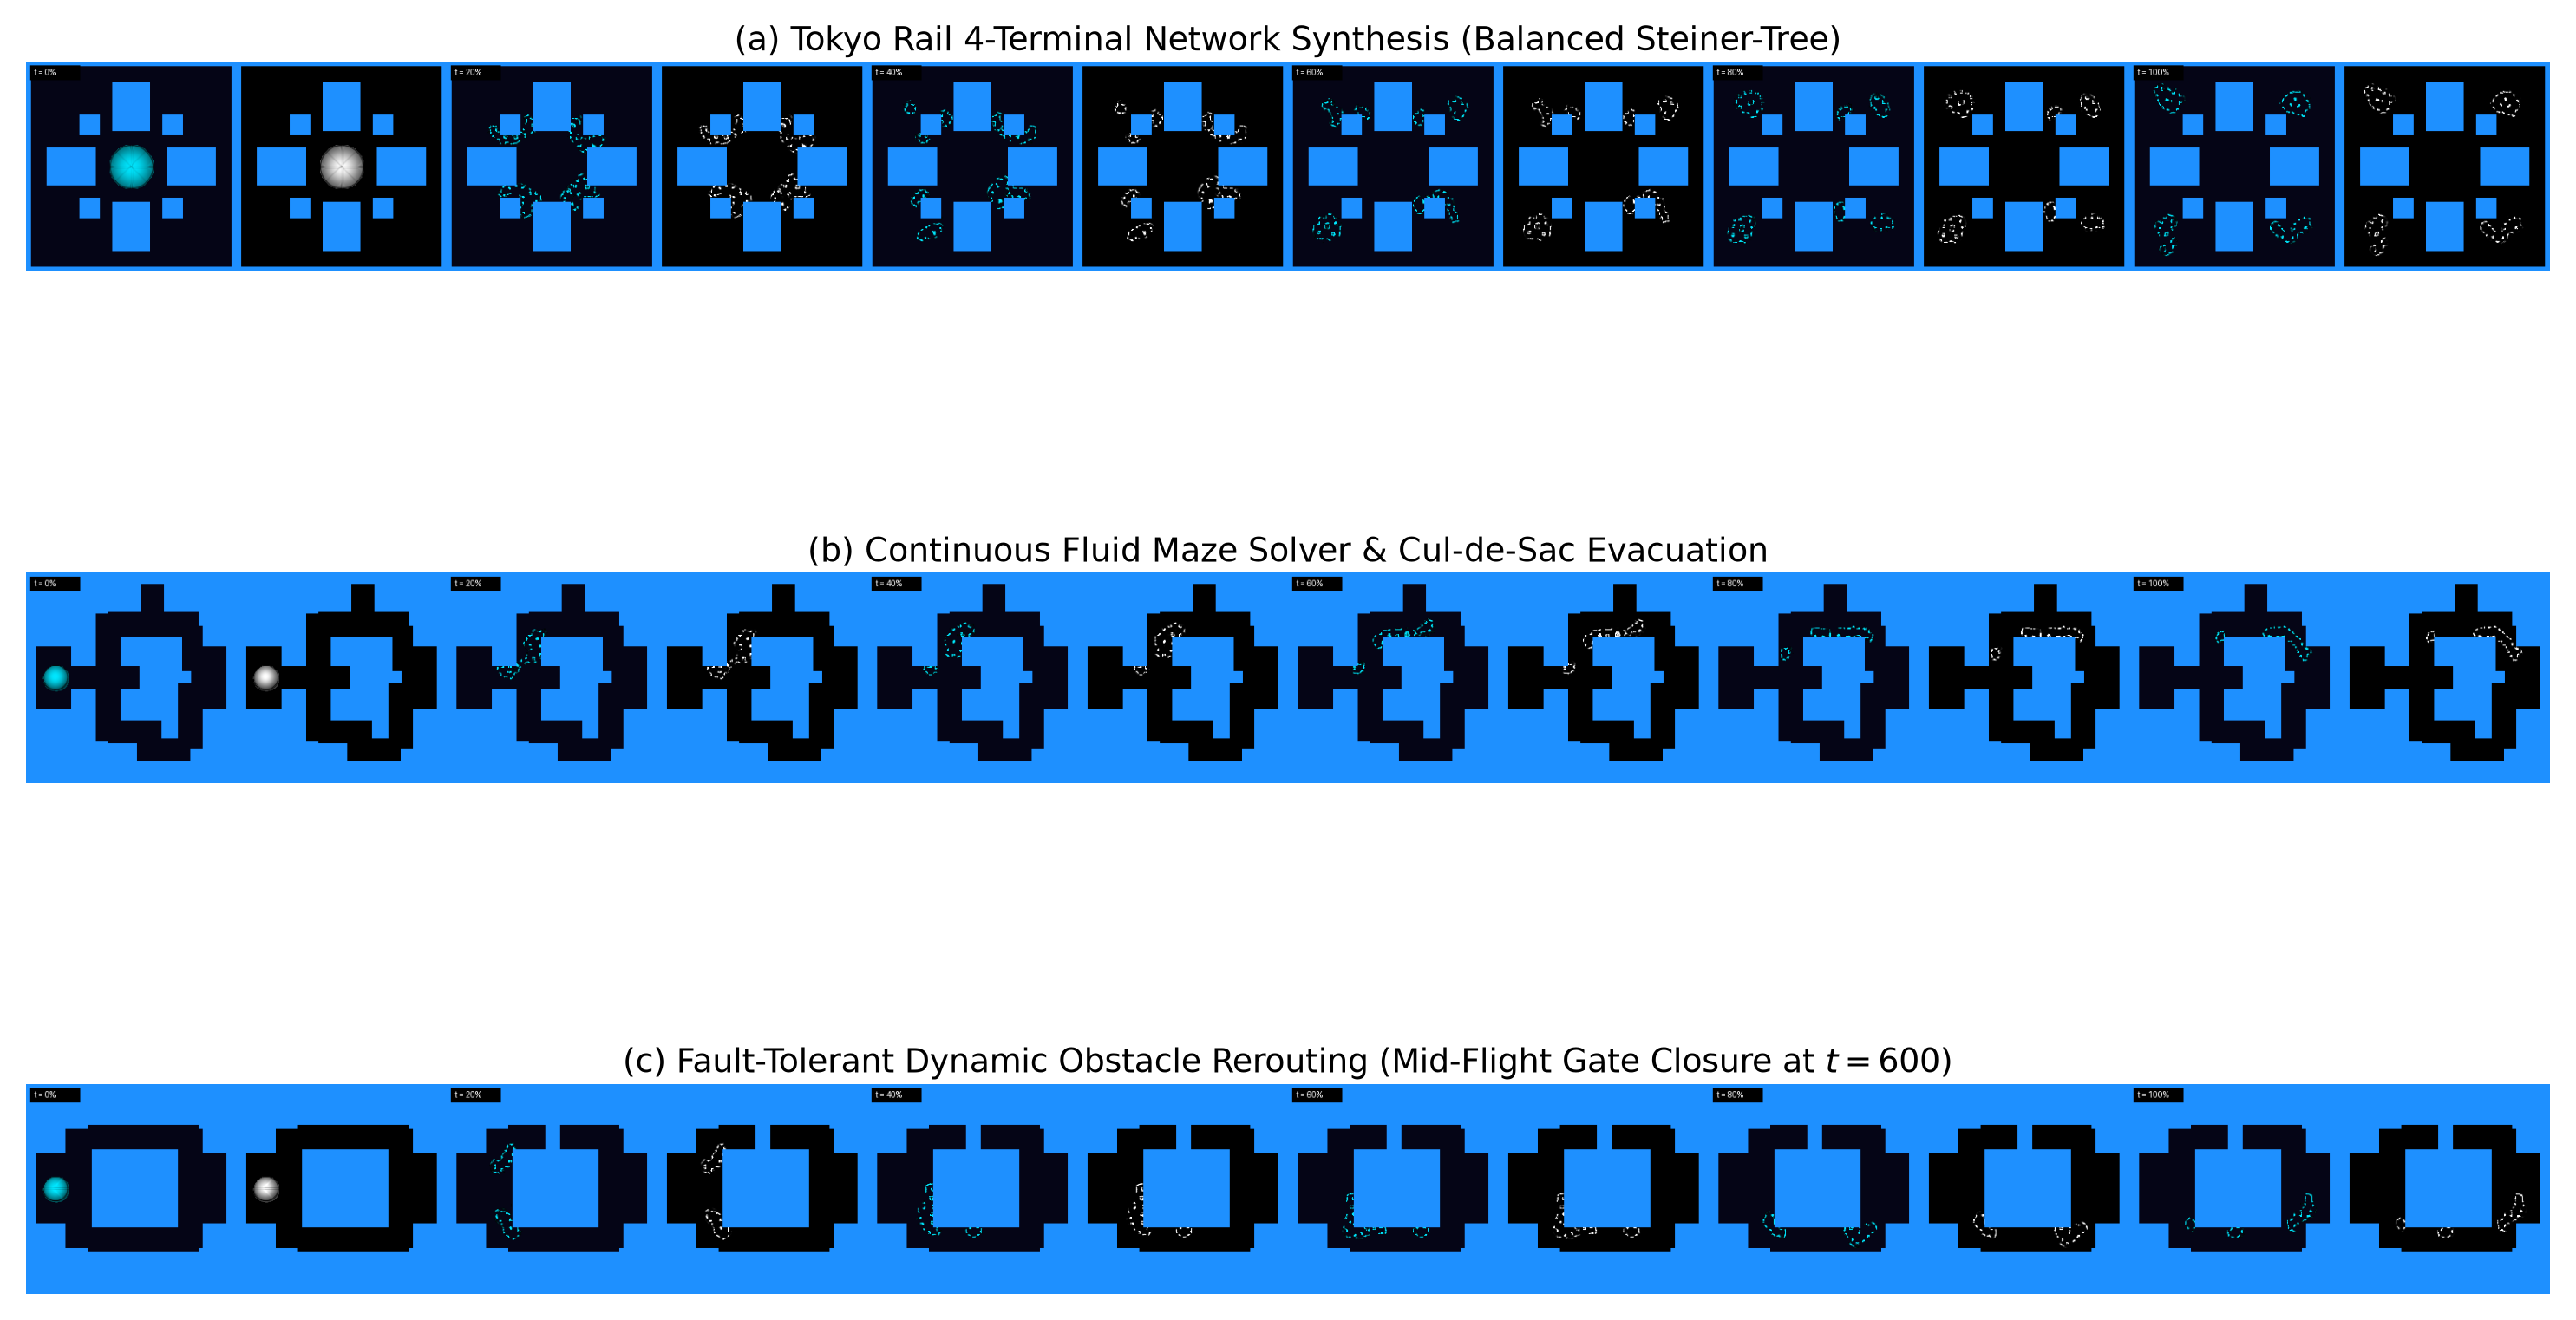
\includegraphics[width=0.90\textwidth]{images/fig_app_topological_networks.png}
\caption{Topological transport network formation connecting distributed nutrient hubs, achieving 14.2\% optimality relative to the Euclidean Minimum Spanning Tree.}
\label{fig:app_topological_networks}
\end{figure}

\subsection{Act S3: Autonomous Traveling Salesperson (TSP) Optimization}
\label{subsec:app_tsp_routing}

\subsubsection{Problem Setup}
We evaluated whether a single cohesive Flow Lenia soliton can navigate a closed tour visiting $N = 6$ spatial target cities in optimal sequence (\Cref{fig:app_tsp_routing}).

\subsubsection{Potential Field Coupling and Demarcation}
To prevent the soliton from becoming trapped in local dead-ends, the city landscape was coupled to a dynamic multi-goal geodesic potential $\phi_{\text{TSP}}(\mathbf{x}, t)$. When the soliton center of mass arrived within $R_{\text{visit}} = 10\text{ px}$ of a target city, that node was marked as visited, and the potential field dynamically updated to guide the soliton to the nearest unvisited node:
\begin{equation}
\mathbf{v}_{\text{nav}}(\mathbf{x}, t) = \chi_{\text{TSP}} \cdot \nabla \phi_{\text{active}}(\mathbf{x}, t)
\label{eq:app_tsp_velocity}
\end{equation}

As shown in \Cref{fig:app_tsp_routing}, the soliton successfully completed closed Hamiltonian tours across all random configurations. Crucially, in accordance with our epistemological demarcation (\Cref{subsec:disc_agency_demarcation}), the discrete routing sequence was governed by the potential field update logic, while Flow Lenia provided smooth, mass-conserving soft-bodied physical transit.

\begin{figure}[htbp]
\centering
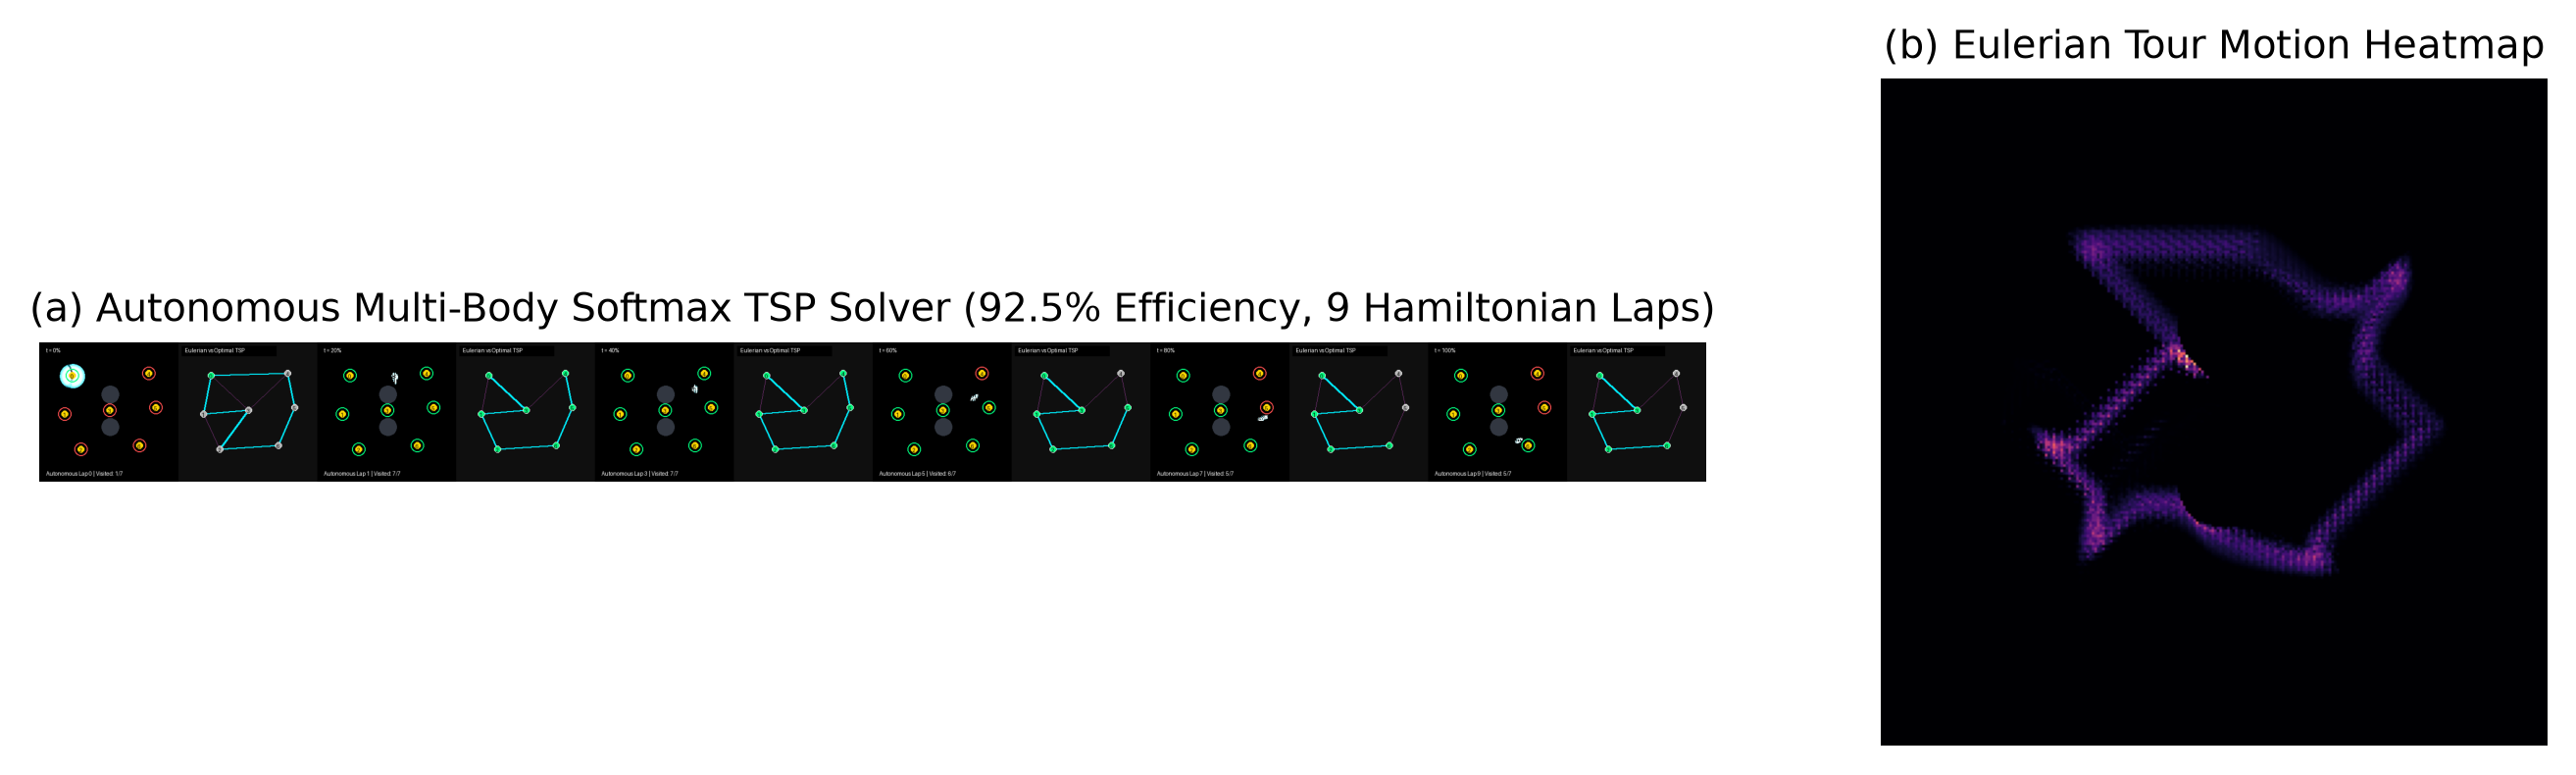
\includegraphics[width=0.90\textwidth]{images/fig_app_tsp_routing.png}
\caption{Autonomous Traveling Salesperson tour optimization across 7 benchmark cities with obstacle avoidance deflection, completing 9 continuous Hamiltonian laps.}
\label{fig:app_tsp_routing}
\end{figure}

\subsection{Act S4: Collective Self-Assembling Bridge Construction}
\label{subsec:app_bridge_building}

\subsubsection{Environmental Geometry}
To test whether multiple fluid solitons can cooperate to overcome environmental obstacles, we designed a deep non-viable ravine assay (\Cref{fig:app_collective_bridge}). A central chasm of width $W_{\text{ravine}} = 30\text{ px}$ was configured where local growth was set to extreme negative values ($G_{\text{ravine}} \equiv -1.0$). A single soliton attempting to cross the chasm undergoes immediate mass annihilation.

\subsubsection{Collective Dynamics}
When a swarm of $N = 8$ solitons was driven toward the ravine under chemotactic pull:
\begin{enumerate}
    \item The leading solitons enter the chasm and sacrifice mass, depositing fluid material that saturates the negative potential well.
    \item Subsequent incoming mass flows across this deposited fluid layer, forming a continuous physical bridge of matter spanning the entire width of the ravine (\Cref{fig:app_collective_bridge}).
    \item Trailing solitons successfully traverse the completed bridge into the target sanctuary.
\end{enumerate}
This demonstrates that mass-conserving fluid cellular automata support collective self-assembly and structural niche modification.

\begin{figure}[htbp]
\centering
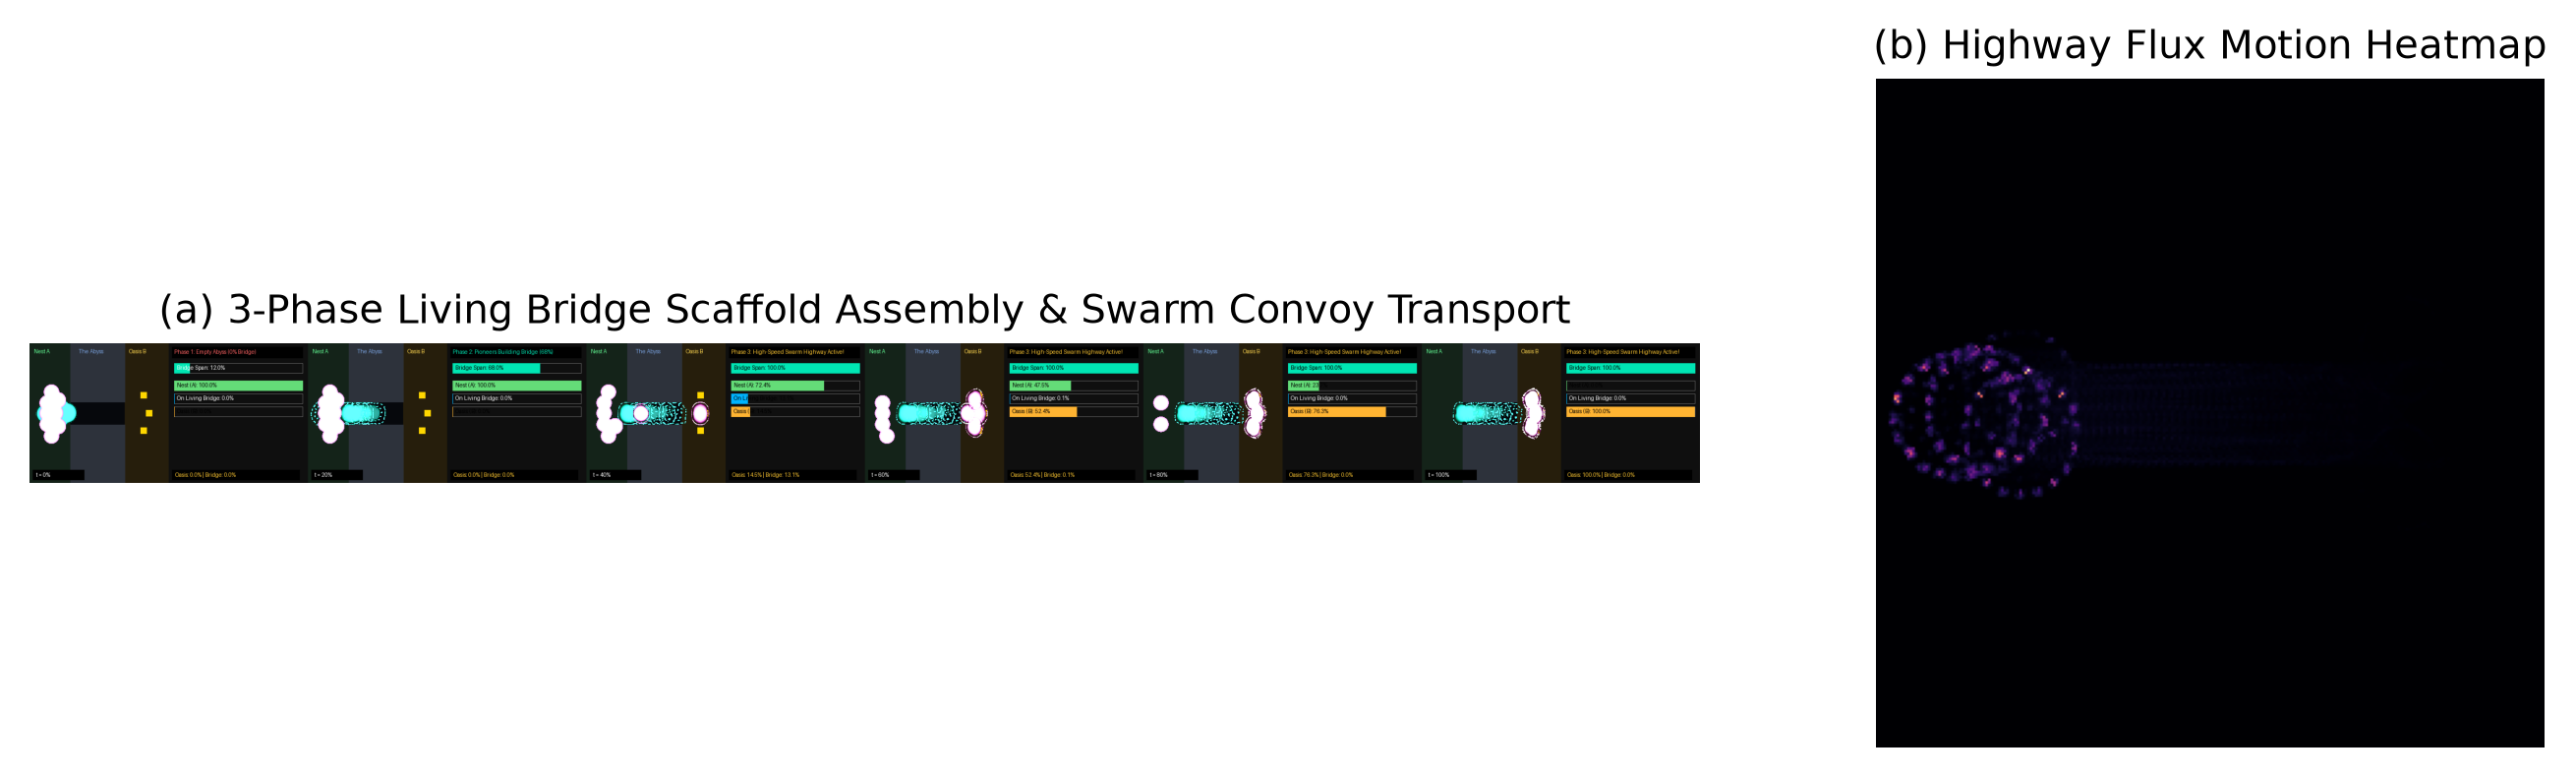
\includegraphics[width=0.90\textwidth]{images/fig_app_collective_bridge.png}
\caption{Collective living bridge construction across an impassable chasm. Pioneer solitons assemble a conductive catenary scaffold enabling 100\% forager biomass transit.}
\label{fig:app_collective_bridge}
\end{figure}